\documentclass[aspectratio=169]{Beamer} % Retire o aspectratio para adaptar a projetores antigos
\usepackage[utf8]{inputenc}		% Codificação do documento (conversão automática dos acentos)
\usepackage{color}				% Controle das cores
\usepackage{graphicx}			% Inclusão de gráficos
\usepackage[brazil]{babel}		% Idioma do documento
\usepackage{float} 				% Fixa tabelas e figuras no local exato
\usepackage{subfig}				% para inserir mais figuras
\usepackage{amsmath}			% para alguns formatos de equações
\usepackage{amssymb}			% para mais símbolos
\usepackage{animate}			% para gifs
\usepackage{pdflscape}			% Pdf landscape
\usepackage{pgfplots}
\usepackage{pgfplotstable}
\usepackage{tikz}
\usepackage{forest}
\usepackage{amsmath}
\usepackage{tabularx}

\usetikzlibrary{trees}
\usetikzlibrary{fit,shapes.arrows,positioning}

\tikzset{marrow/.style={midway,red,sloped,fill, minimum height=3cm, single arrow, single arrow
            head extend=.5cm, single arrow head indent=.25cm,xscale=0.3,yscale=0.15,
            allow upside down}}
%------	%------	%------	%------	%------	%------	%------	
\title[Especialização em Ciência de Dados e Big Data - ECD]{Análise de sentimentos em avaliações de clientes do \textit{e-commerce} nacional e comparação de métodos tradicionais de \textit{machine learning} com Redes Neurais \textit{Long Short Term Memory} (LSTM)}
%------	%------	%------	%------	%------	%------	%------	
\author[Carlos Magno de Brito]{{\Large Carlos Magno Santos Ribeiro de Brito}}
%------	%------	%------	%------	%------	%------	%------	
\institute[UFBA]{{\large Universidade Federal da Bahia}\\Instituto de Matemática e Estatística}
%------	%------	%------	%------	%------	%------	%------	
\date[UFBA 2023]

\logo{\includegraphics[width=0.8 cm]{logo_ufba.eps}}
\newcommand{\nologo}{\setbeamertemplate{logo}{}} % command to set the logo to nothing
%------	
\usetheme{CambridgeUS}
\usecolortheme{beaver}
%------ %------	%------	%------	%------	%------	%------
\usefonttheme[onlymath]{serif}	
%------ %------	%------	%------	%------	%------	%------
\begin{document}
% Definindo a capa
\frame{\titlepage}
% Definindo o sumário dividido na quantidade de slides necessária
\frame{\tableofcontents[part=1]}
% \frame{\tableofcontents[part=2]}
%------ %------	%------	%------	%------	%------	%------		
\part{1}
\section{Introdução}
\nologo
\frame{
    \frametitle{Introdução}
    \begin{itemize}
        \item O \textit{e-commerce} anualmente movimenta bilhões de dolares no mundo e está em franca expansão; \vskip1cm
        \item Os empreendimentos estão cada vez mais adotando tecnologias diversas em suas plataforma, inclusive lançando mão da ciência de dados para isso;\vskip1cm
        \item Para se manter competitiva e sólida neste mercado, uma empresa precisa de planejamento, inovação e, principalmente, entender sobre as necessidades dos clientes e como fidelizá-los;\vskip1cm
        \item Uso de métodos do \textit{machine learning} e redes neurais surgem como opção para análise dos dados;
    \end{itemize}
}
\frame{
    \frametitle{Introdução}
    \begin{itemize}
        \item Usuários plenamente satisfeitos e/ou insatisfeitos tendem a avaliar corretamente o produto, porém, fora dessa faixa é encontrada muita inconsistência;\vskip1cm
        \item A depender do contexto, faz-se necessário utilizar métodos que sejam mais eficazes e consigam ter um \textit{tradeoff} entre tempo de processamento/acurácia satisfatório;\vskip1cm
        \item Foram utilizados cinco métodos tradicionais de aprendizado de máquina (Regressão logística, Naive Bayes, XGBoost, LightGBM e Florestas Aleatórias) e um modelo de rede neural artificial (LSTM) para fins comparativos.
    \end{itemize}
}
\subsection{Objetivos}
\frame{
    \frametitle{Objetivos}
    \begin{block}{Objetivo principal}
        Realizar análise com base de dados real sobre melhores modelos para se utilizar em estudo de satisfação dos consumidores em um comércio eletrônico
    \end{block}
    \begin{alertblock}{Objetivo secundário}
        \begin{itemize}
            \item Ponderar com a relação de eficiência \textit{versus} custo;
            \item Obter melhor precisão na classificação dos reviews com base nos comentários;
            \item Aplicar conceitos diversos da ciência/engenharia de dados, como por exemplo a mineração de texto, pré processamento e pós processamento de dados;
            \item Apresentar uma visão geral sobre o comércio eletrônico (e-commerce), sua evolução e importância no mercado brasileiro.
        \end{itemize}
    \end{alertblock}
}

\subsection{Justificativa}
\frame{
    \frametitle{Justificativa}
    Dentre as principais justificativas para o estudo dos \textit{e-commerces}, tem-se:\vskip0.5cm
    \begin{itemize}
        \item A análise de dados com essas técnicas pode ser feita de forma automatizada, reduzindo custos e tempo de processamento em comparação com análises manuais.;\vskip1cm
        \item Com essas técnicas é possível prever o comportamento dos consumidores, ajudando as empresas a tomarem decisões estratégicas;\vskip1cm
        \item A análise de dados com \textit{machine learning} e redes neurais pode ser aplicada em diferentes áreas do e-commerce, como marketing digital, o seu uso pode ajudar o negócio a otimizar o seu sistema logístico, reduzindo os custos de entrega e aumentando a satisfação dos clientes.
    \end{itemize}
}

\section{Materiais}
\frame{
    \frametitle{Tipo de pesquisa e descrição dos dados}
    \begin{itemize}
        \item A Olist é uma startup brasileira que atua no segmento de E-commerce por meio de marketplace.
        \item A empresa concentra vendedores que desejam anunciar em marketplaces como Mercado Livre, B2W, Via Varejo, Amazon, entre outros.
        \item A Olist concentra os produtos de todos os vendedores em uma loja única que fica visível ao consumidor final.
        \item Atualmente, a empresa reúne mais de 800 colaboradores e mais de 9 mil lojistas, além de 2 milhões de consumidores únicos.
        \item A base de dados escolhida para análise descreve a rotina de compra de um E-commerce e contém diversas informações sobre os produtos, como nome, preço, descrição, nota atribuída, comentários e local de compra.
    \end{itemize}
}

\frame{
    \frametitle{Tipo de pesquisa e descrição dos dados}
    \begin{itemize}
        \item A base utilizada é uma base pública disponível no Kaggle e publicada pela Olist;\vskip1cm
        \item A análise se concentra especificamente nos comentários avaliativos e nas notas dadas pelos clientes;\vskip1cm
        \item A tabela com possui 100 mil linhas depois de tratada com as informações pertinentes ao comentário avaliativo e à nota referente;\vskip1cm
        \item Os atributos originais utilizados são \textit{review\_score} e \textit{review\_comment\_message} da tabela \textit{olist\_order\_review}
    \end{itemize}
}

\frame{
    \frametitle{Exemplo}
    \begin{figure}[H]
        \centering
        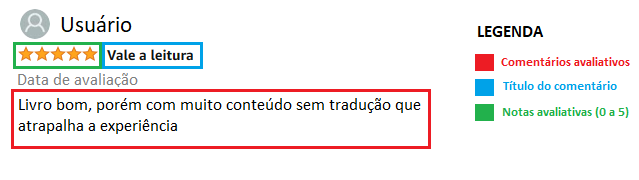
\includegraphics[width=\linewidth, scale=0.7]{../TCC/figs/review_ex.png}
        \caption{Exemplo de como é efetuada a avaliação}
        \label{fig:review_ex}
    \end{figure}
}

\frame{
    \frametitle{Tipo de pesquisa e descrição dos dados}
    \begin{figure}[H]
        \centering
        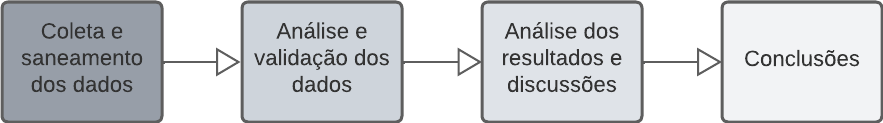
\includegraphics[width=\linewidth, scale=0.6]{../TCC/figs/process_diagram.png}
        \caption{Fluxograma do trabalho}
        \label{fig:process}
    \end{figure}
}
\frame{
    \frametitle{Exemplo da tabela usada}
    \begin{table}[H]
        \small
        \begin{tabular}{ccccc}
            \hline
            { }     & { review\_id}   & { order\_id}   & { review\_comment\_title} & { review\_comment\_message} \\ \hline
            { type} & { hash}         & { hash}        & { string|null}            & { string|null}              \\
            { ex}   & { da79b0a377eb} & { df73dbeba33} & { bom, mas}               & { atende às expectativas}   \\ \hline
        \end{tabular} \ldots
        \newline
        \vspace*{0.5 cm}
        \newline
        \begin{tabular}{cccc}
            \hline
            { }     & { review\_score} & { review\_creation\_date} & { review\_answer\_timestamp} \\ \hline
            { type} & { number}        & { datestring}             & { datestring}                \\
            { ex}   & { 3}             & { 2018-01-18 00:00:00}    & { 2018-01-18 21:00:00}       \\ \hline
        \end{tabular}
        \caption{Esquema da tabela \textit{olist\_order\_review}}
        \label{tab:review}
    \end{table}
}
\frame{
    \frametitle{Dataset utilizado}
    \begin{figure}[H]
        \centering
        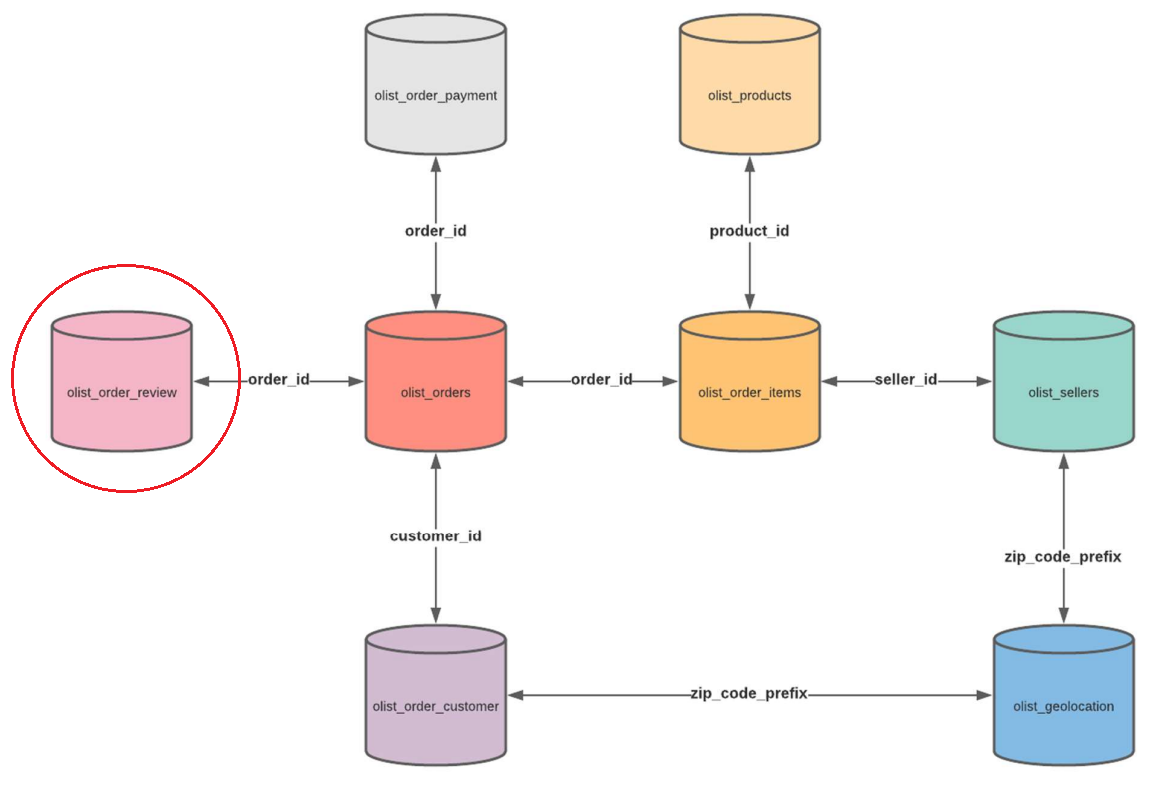
\includegraphics[scale=0.35]{../TCC/figs/database_schema.png}
        \caption{Esquemas do dataset publicado pelo Olist, adaptado pelo autor (2022)}
        \label{fig:dataset_schema}
    \end{figure}
}

\frame{
    \frametitle{Dataset transformado para uso}
    \begin{table}[H]
        \centering
        \begin{tabular}{cccc}
                    & index  & text               & label   \\\hline\hline
            type    & bigint & string             & boolean \\\hline
            exemplo & 1      & produto muito ruim & 0
        \end{tabular}
        \caption{Esquema de geração do \textit{data\_bin}}
        \label{tab:bin}
    \end{table}

    \begin{table}[H]
        \centering
        \begin{tabular}{cccc}
                    & index  & text              & label  \\\hline\hline
            type    & bigint & string            & number \\\hline
            exemplo & 2      & produto muito bom & 4
        \end{tabular}
        \caption{Esquema de geração do \textit{data\_gen}}
        \label{tab:gen}
    \end{table}

}
\frame{
    \begin{itemize}
        \item Os databases em formato CSV foram extraídos e exportados para leitura e armazenamento em diferentes variáveis.
        \item Itens duplicados, com valores nulos e valores discrepantes foram removidos.
        \item Separou-se dois \textit{datasets} contendo informações dos comentários dos clientes (\textit{review\_comment\_message}) e da sua nota de avaliação (\textit{review\_score}).
        \item Para o \textit{data\_bin} tem-se comentários associados categoricamente com valores binários (0 e 1) a partir das notas, com o valor atribuído de 0 para o intervalo $(0,2]$ e de 1 para o intervalo de $(2,5]$.
        \item No \textit{data\_cat} tem-se apenas os comentários e os reviews numéricos de 1 a 5.
        \item Os dados de entrada (comentários) foram transformados em uma lista de números por meio de um processo de tokenização;
        \item Ambas as bases são removidos os valores nulos.
    \end{itemize}
}

\subsubsection{Máquina para processamento}
\frame{
    \frametitle{Máquina para processamento}
    Todos os métodos foram executados em fila, sequencialmente entre eles, onde cada um deles foi executado em ordem, um de cada vez e de maneira procedural.

    A máquina utilizada para todos eles foi o laptop Dell G3 com processador Intel Core i7 de 10ª geração, 16GB de RAM, 512GB de SSD e placa de vídeo NVIDIA RTX 2060 com 6GB de memória dedicada, incluindo o sistema operacional Windows 11 com WSL 2 instalado e Ubuntu 20.04 como ambiente de execução para as ferramentas de teste de software usadas.
}



\section{Métodos}
\frame{
    \frametitle{Comparação dos métodos utilizados}
    Com base nos resultados e literatura, a tabela a seguir foi elaborada com as principais vantagens/características de cada método utilizado:
    \begin{figure}[H]
        \centering
        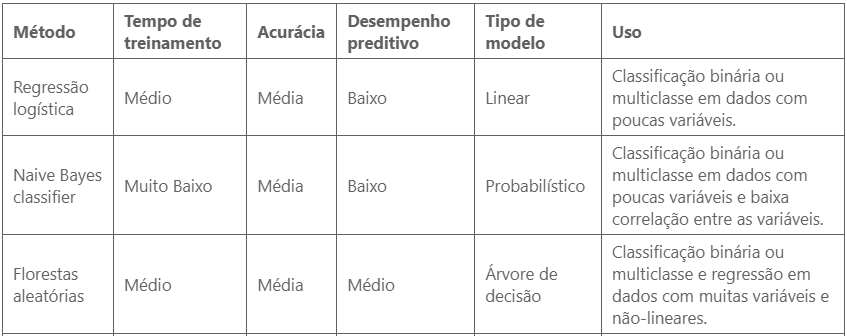
\includegraphics[scale=0.55]{../TCC/figs/table_pt1.png}
        \label{fig:table_pt1}
    \end{figure}
}

\frame{
    \frametitle{Comparação dos métodos utilizados}
    Com base nos resultados e literatura, a tabela a seguir foi elaborada com as principais vantagens/características de cada método utilizado:
    \begin{figure}[H]
        \centering
        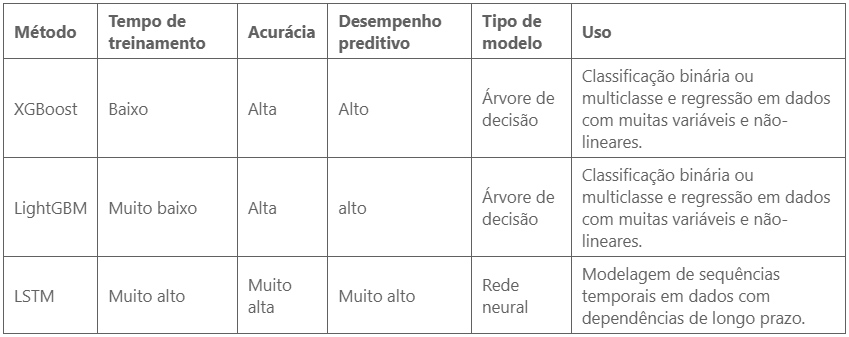
\includegraphics[scale=0.55]{../TCC/figs/table_pt2.png}
        \label{fig:table_pt2}
    \end{figure}
}
\section{Resultados}
\frame{
    \frametitle{Distribuição}
    \begin{figure}[H]
        \centering
        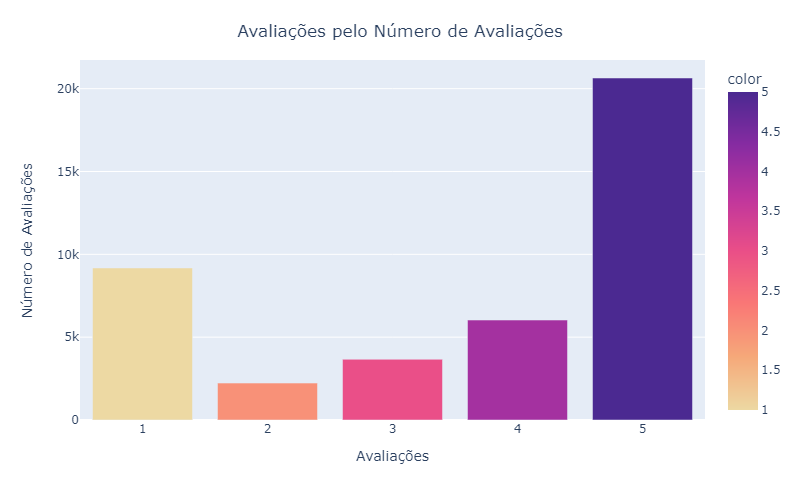
\includegraphics[trim={0cm 2cm 3cm 2cm},clip,scale=0.4]{../TCC/figs/eval.png}
        \caption{Distribuição das avaliações}
        \label{fig:evalDistribution}
    \end{figure}
}

\frame{
    \begin{itemize}
        \item Nota 1 corresponde às piores avaliações, nota 5 às melhores;\vskip0.7cm
        \item A distribuição das avaliações apresenta uma forma de "J", com grande quantidade de notas 5, 4 e 1, e pequena quantidade de notas 2 e 3;\vskip0.7cm
        \item Isso pode ocorrer porque clientes extremamente satisfeitos ou insatisfeitos são mais propensos a deixar avaliações;\vskip0.7cm
        \item Além disso, clientes que tiveram uma experiência neutra podem não se sentir motivados a deixar uma avaliação, o que resulta em uma concentração menor de avaliações com notas médias;\vskip0.7cm
        \item A distribuição em forma de "J" pode fornecer informações importantes sobre a satisfação do cliente e a qualidade do produto.

    \end{itemize}
}
\frame{
    \frametitle{Distribuição}
    \begin{figure}[H]
        \centering
        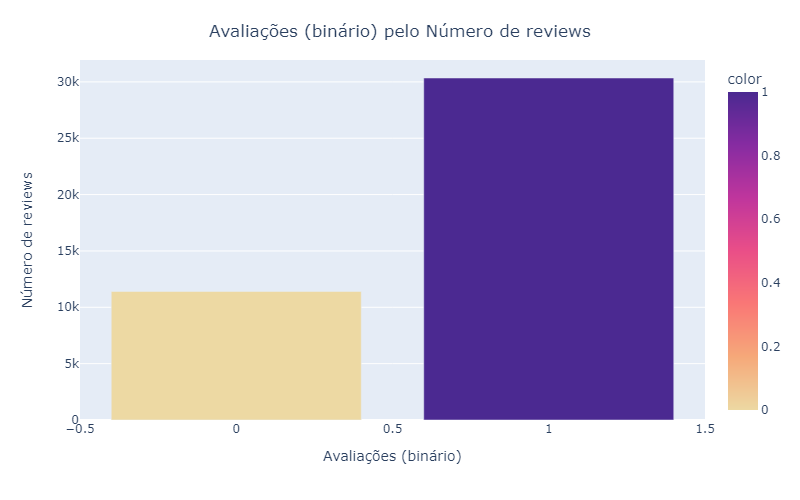
\includegraphics[trim={0cm 2cm 3cm 2cm},clip,scale=0.4]{../TCC/figs/bin_eval.png}
        \caption{Distribuição das avaliações binárias}
        \label{fig:binEvalDistribution}
    \end{figure}
}

\frame{
    \frametitle{Word Cloud}
    \begin{figure}[H]
        \centering
        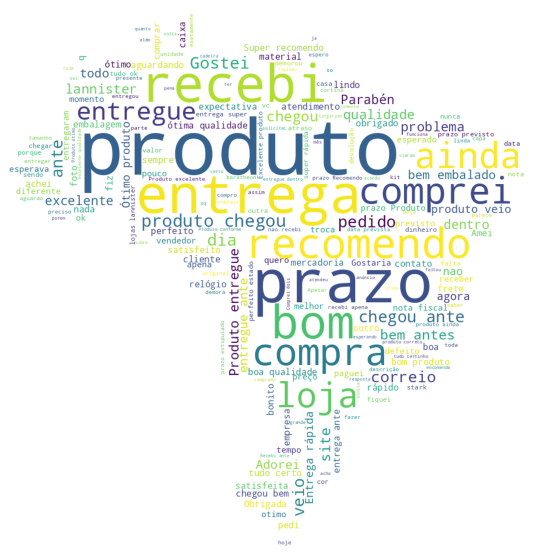
\includegraphics[scale=0.3]{../TCC/figs/word_cloud.png}
        \caption{Nuvem de palavras destacando os principais termos utilizados}
        \label{fig:wordCloud}
    \end{figure}
}

\frame{
    \begin{itemize}
        \item Nuvem de palavras é feita com as entradas de dados, que são os principais termos usados nos comentários, excluindo as \textit{stopwords};\vskip0.7cm
        \item Essa técnica visual pode ser usada em vários campos, incluindo análise de sentimentos, mineração de opiniões, análise de redes sociais, pesquisa de mercado e análise de feedback de clientes como o caso em específico\vskip0.7cm
        \item Além disso, por ser uma forma visualmente atraente de resumir informações e destacar pontos importantes, é bastante útil para relatórios e análises.
    \end{itemize}
}

\frame{
    \frametitle{Acurácias dos modelos de ML}
    \begin{table}[H]
        \centering
        \begin{tabular}{l|ccccc}
            \hline
            { modelo}      & { Reg. Logística} & { F. Aleatórias} & { XGBoost} & { Naive Bayes} & LightGBM \\ \hline\hline
            { treino (\%)} & { 73.9}           & { 99.6}          & { 93.5}    & { 74.0}        & 86.7     \\\hline
            { teste (\%)}  & { 73.3}           & { 78.2}          & { 82.1}    & { 74.0}        & 81.3
        \end{tabular}
    \end{table}
}

\frame{
    \frametitle{Acurácia da rede neural LSTM vs Epochs}
    \begin{figure}[H]
        \centering
        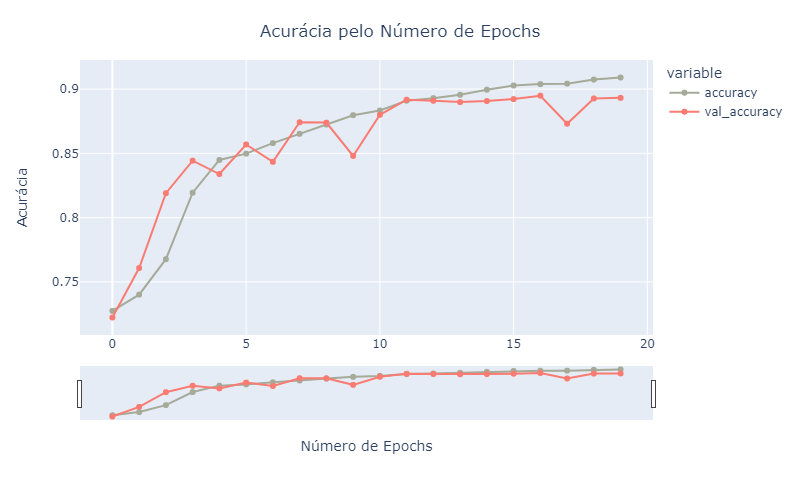
\includegraphics[scale=0.4]{../TCC/figs/lstm_acuracy.png}
        \caption{Relação acurácia por \textit{epochs}}
        \label{fig:lstmacuracy}
    \end{figure}
}

\frame{
    \frametitle{Acurácias comparadas}
    \begin{figure}[H]
        \centering
        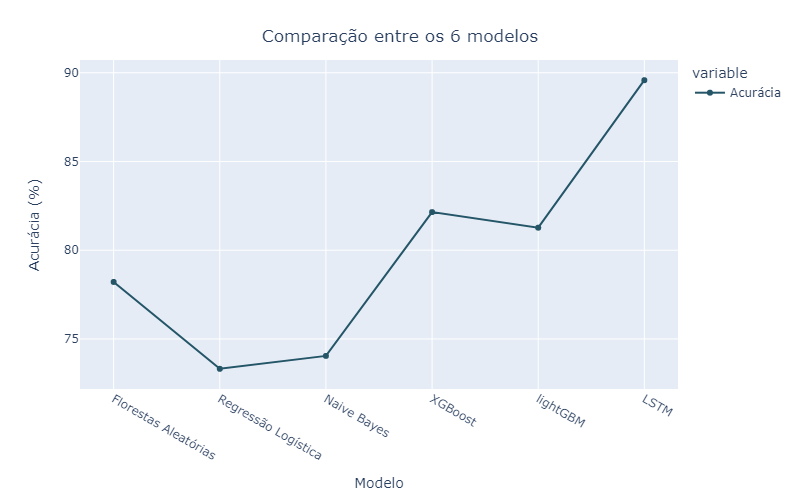
\includegraphics[scale=0.35]{../TCC/figs/comparative.png}
        \caption{Comparação de acurácia entre modelos}
        \label{fig:comparative}
    \end{figure}
}

\frame{
    \frametitle{\textit{Tradeoff}}
    \begin{table}[H]
        \centering
        \small
        \begin{tabular}{c|cccccc}
            \hline
            { modelo}        & { Reg. Logística} & { F. Aleatórias} & { XGBoost} & { Naive Bayes} & LightGBM & LSTM \\ \hline \hline
            { Tempo (s)}     & { 21.5}           & { 1.5}           & { 3.0}     & { 0.1}         & {1.5}    & 1500 \\ \hline
            { Acurácia (\%)} & { 73.3}           & { 78.2}          & { 82.1}    & { 74.0}        & 81.3     & 90.0 \\
        \end{tabular}
        \caption{Tempo de execução/Acurácia dos modelos avaliados em teste}
        \label{tab:time}
    \end{table}
}

\frame{
    \frametitle{Matriz de confusão}
    \begin{figure}[H]
        \centering
        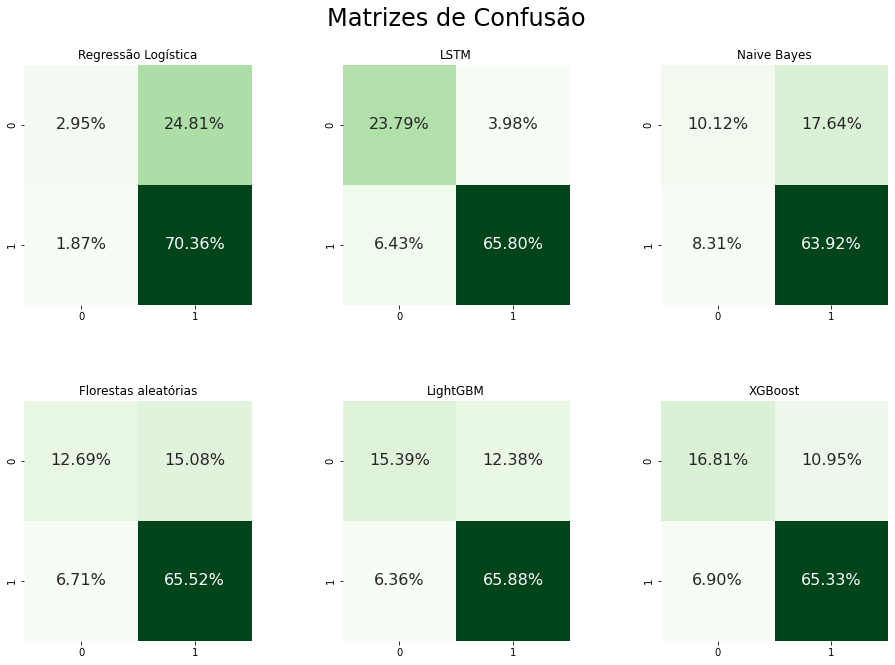
\includegraphics[scale=0.3]{../TCC/figs/confusion.png}
        \caption{Matrizes de confusão dos modelos utilizados}
        \label{fig:roccurve}
    \end{figure}
}

\frame{
    \frametitle{Curva HOC}
    \begin{figure}[H]
        \centering
        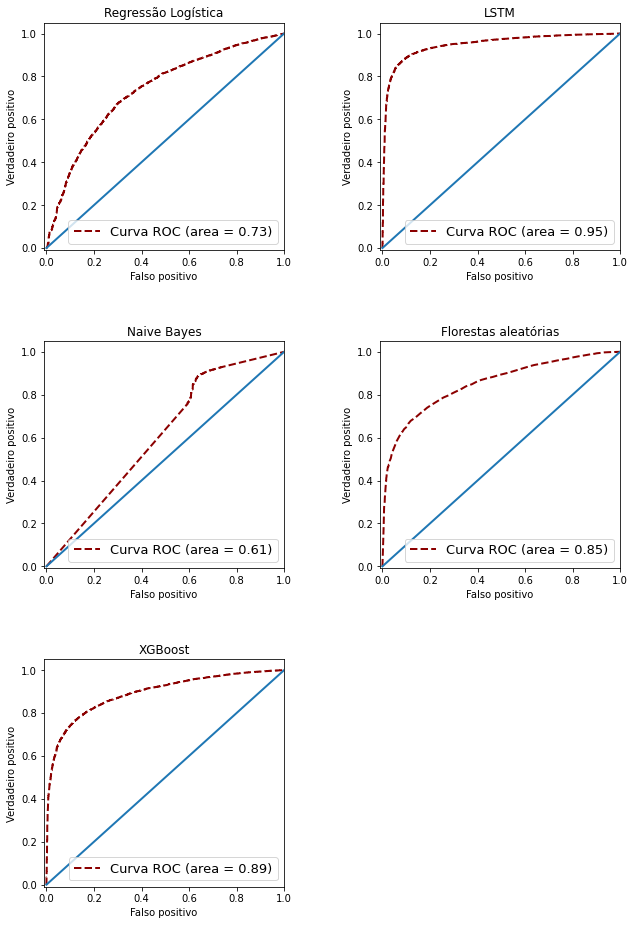
\includegraphics[scale=0.25]{../TCC/figs/roc.png}
        \caption{Curvas ROC dos modelos utilizados}
        \label{fig:mconfusion}
    \end{figure}
}




\section{Conclusões}
\frame{
    \frametitle{Conclusões}
    \begin{itemize}
        \item A Rede neural LSTM apresentou a melhor performance entre os algoritmos de machine learning avaliados, com acurácia de $90\%$ e maior capacidade de distinguir entre as classes, indicado pela área sob a curva ROC.

        \item XGBoost e LightGBM também apresentaram resultados promissores, com acurácia de $\approx 82\%$ e área sob a curva ROC de 0,89, mas cometeu mais erros na classificação de algumas amostras do que a LSTM.

        \item Regressão logística e Naive Bayes tiveram as piores performances, com acurácias de $73\%$ e $74\%$, respectivamente, e áreas sob a curva ROC menores do que os outros modelos avaliados.
    \end{itemize}
}
\frame{
    \frametitle{Conclusões}
    \begin{itemize}
        \item É necessário encontrar um equilíbrio entre a rapidez da resposta e a precisão do modelo em muitas aplicações em tempo real.

        \item A escolha do modelo ideal depende de vários fatores, como o tamanho dos dados, a complexidade do problema e a disponibilidade de recursos de computação.

        \item Modelos mais simples, como regressão logística ou Naive Bayes, têm tempos de processamento menores, mas podem ter uma acurácia menor, enquanto modelos mais complexos, como redes neurais, podem ter uma acurácia muito alta, mas exigem uma grande quantidade de tempo de processamento. As Florestas Aleatórias, LightGBM e o XGBoost são modelos intermediários que podem ser mais adequados para muitas aplicações.
    \end{itemize}
}

\frame{
    \frametitle{Conclusões}
    \begin{itemize}
        \item O XGBoost possui vantagens em relação a redes neurais, como a capacidade de lidar com dados heterogêneos e faltantes de forma eficiente, e a simplicidade e rapidez no treinamento.
        \item O XGBoost também é interpretável, permitindo a identificação das variáveis mais importantes para a classificação dos dados.
        \item O LightGBM é mais rápido que o XGBoost, usando uma técnica de otimização chamada "histogram-based" para encontrar os melhores pontos de divisão de árvore, permitindo o processamento de conjuntos de dados maiores e mais complexos em menos tempo.
    \end{itemize}
}

\frame{
    \frametitle{Conclusões}
    \begin{itemize}
        \item O LightGBM usa menos memória do que o XGBoost, utilizando uma técnica de amostragem chamada "leaf-wise" em vez de "level-wise", permitindo criar árvores mais profundas com menos nós.
        \item O LightGBM tem melhor desempenho em conjuntos de dados esparsos, sendo melhor em lidar com eles devido à técnica de exclusão de zeros para reduzir a sobrecarga computacional em recursos esparsos.
        \item A LSTM, por sua vez, é capaz de lidar com dados sequenciais e com dependências de longo prazo, o que pode ser um desafio para algoritmos tradicionais de aprendizado de máquina.
    \end{itemize}
}

\frame{
    \frametitle{Conclusões}
    \begin{itemize}
        \item A LSTM também é capaz de aprender padrões complexos em dados sequenciais sem a necessidade de engenharia manual de características, tornando-se uma escolha popular em tarefas de processamento de linguagem natural e análise de séries temporais.
        \item A LSTM é capaz de lidar com dados de entrada de diferentes tipos e tamanhos, como sequências de palavras, imagens e dados numéricos.
        \item Para análise de sentimentos em reviews de usuários, a LSTM pode ser mais vantajosa do que o XGBoost devido à sua capacidade de capturar dependências de longo prazo nos dados sequenciais e trabalhar eficientemente com dados sequenciais.
    \end{itemize}
}

\end{document}